Image recognition is an important part in Computer Vision which includes many advanced machine learning techniques. A pattern recognition system (PRS) is an automatic system that aims at classifying the input pattern into a specific class\cite{kpalma2007overview}. An image recognition system
always proceeds in two steps: (1) generate several important features (descriptors or a book of code) (2) use a classifier
to distinguish the patterns with all these features. Compared to our human learning procedures, some prior knowledge should acquired
before the recognition which turns the learning procedure into be a supervised learning.

There are four major methodologies in image recognition:
\begin{itemize}
  \item Statistical approach. Here features are converted into a vector to present the pattern which can be a very easy to handle. This method
        is wildly and intensively used in practice.

  \item Syntactic approach. This method analysis the relationship between features and patterns are described in a hierarchical structure. For example
        (see \figref{sys}), the image on the right hand can be presented as the string ${d b a b c b a b d b a b c b a b}$.The system parses the set of extracted features using a kind of predefined grammar. If the whole features extracted from a pattern can be parsed to the grammar then the system has recognised the pattern. Unfortunately, grammar-based syntactic pattern recognition is generally very difficult to handle.

  \item Template matching. This can be the most intuitive way to localize and identify shapes in an image. Here, the method looks for the parts of the
        image which match the template. For each possible position in the image, it compares with each possible rotation or each possible geometric transformation of the template. According to certain metrics that can measure the similarity of these, the approach returns the most similar one. Since it has to compute all kinds of possibilities, this could be a very computational expensive approach.
  \item Neural networks. The an artificial neural network (ANN) had been used extensively before 2006 for image recognition. In 2006,  G. Hinton introduced "deep learning", a new method that can learning image features with fast unsupervised procedure which led to a revolutionary in image recognition\cite{hinton06}. We will
      discuss this method in details in section \ref{dl}.
\end{itemize}
\begin{figure}
  \centering
  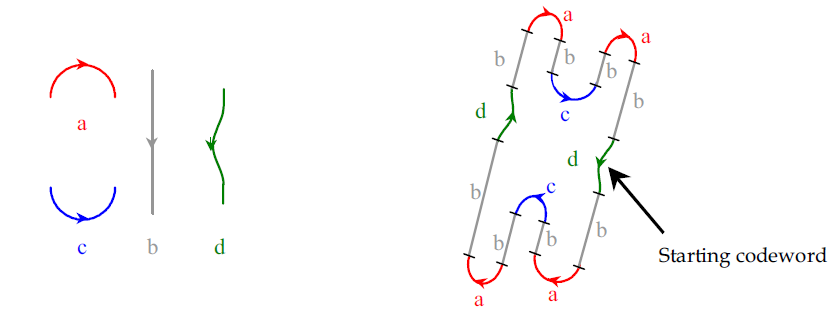
\includegraphics [width=6in] {fig/sys.png}\\
  \caption{Example of syntactic description features}\label{sys}
\end{figure}
There are some simple dependencies when representing the image patterns. One reason why explicitly dealing with image patterns is interesting is because they can be convenient to express many general priors about the world around us, i.e., priors that are not task specific but would be likely to be useful for a learning machine to solve AI tasks\cite{bengio2007scaling}. These general priors can sometime be used to help us design more powerful learners to discover the underlying factors that the data may reveal. Here are some examples of the general-purpose priors:
\begin{itemize}
  \item Smoothness: Assumes that the function $f$ to be learning for evaluation must satisfy that for any two patterns $x,y$, if $x\approx y, f(x)\approx f(y)$.
  %\item Multiple explanatory factors:
  \item A hierarchical organization of explanatory factors: Some patterns are more abstract than the others. These abstract patterns can be defined in terms of other patterns hierarchically.
  %\item Semi-supervised learning:
  %\item Shared factors across tasks
  %\item Manifolds:
  \item Natural clustering: Different values of categorical variables such as object classes are associated with separate manifolds. Humans have named categories and classes because of such statistical structure (discovered by their brain and propagated by their culture), and machine learning tasks often involve predicting such categorical variables.
 % \item Temporal and spatial coherence
  \item Sparsity: For any given observation $x$, only a small fraction of the possible factors are relevant\cite{olshausen1996emergence}. This means just a small fraction of the patterns can represent a image well.
  \item Simplicity of factor dependencies: The good abstract patterns can be related to each other through simple, typically linear combination.This can be seen in many neural networks when the top layer is just linear combination of the hidden units.
\end{itemize}






